\documentclass{article}
\usepackage[margin=1.0in]{geometry}
\usepackage{amsmath, amssymb, mathrsfs}
\usepackage[english]{babel}
\usepackage{graphicx}
\usepackage{enumerate}
\usepackage{listings}
\usepackage{tikz}
\usepackage{epstopdf}
\renewcommand{\vec}[1]{\mathbf{#1}}
\newcommand{\floor}[1]{\left\lfloor #1 \right\rfloor}
\newcommand{\ceil}[1]{\left\lceil #1 \right\rceil}

\title{Machine Learning from Data Assignment 9}
\author{Greg Stewart}
\date{\today}

\begin{document}

\maketitle

\subsection*{1. $8^{th}$ order feature transform.}

The 8th order transform for $\vec{z}$ is given by 

\[
  \vec{z} = 
  \begin{pmatrix}
    1 & L_1(x_1) & L_1(x_2) & L_1(x_1)L_1(x_2) & L_2(x_1) & \cdots & L_1(x_1)L_7(x_2) & L_8(x_2)
  \end{pmatrix}^T
\]

This is a 45 dimensional vector. Thus the transformed data matrix Z will be of dimensions 
(300, 45).

\subsection*{2. Overfitting.}

\begin{figure}[h!]
% 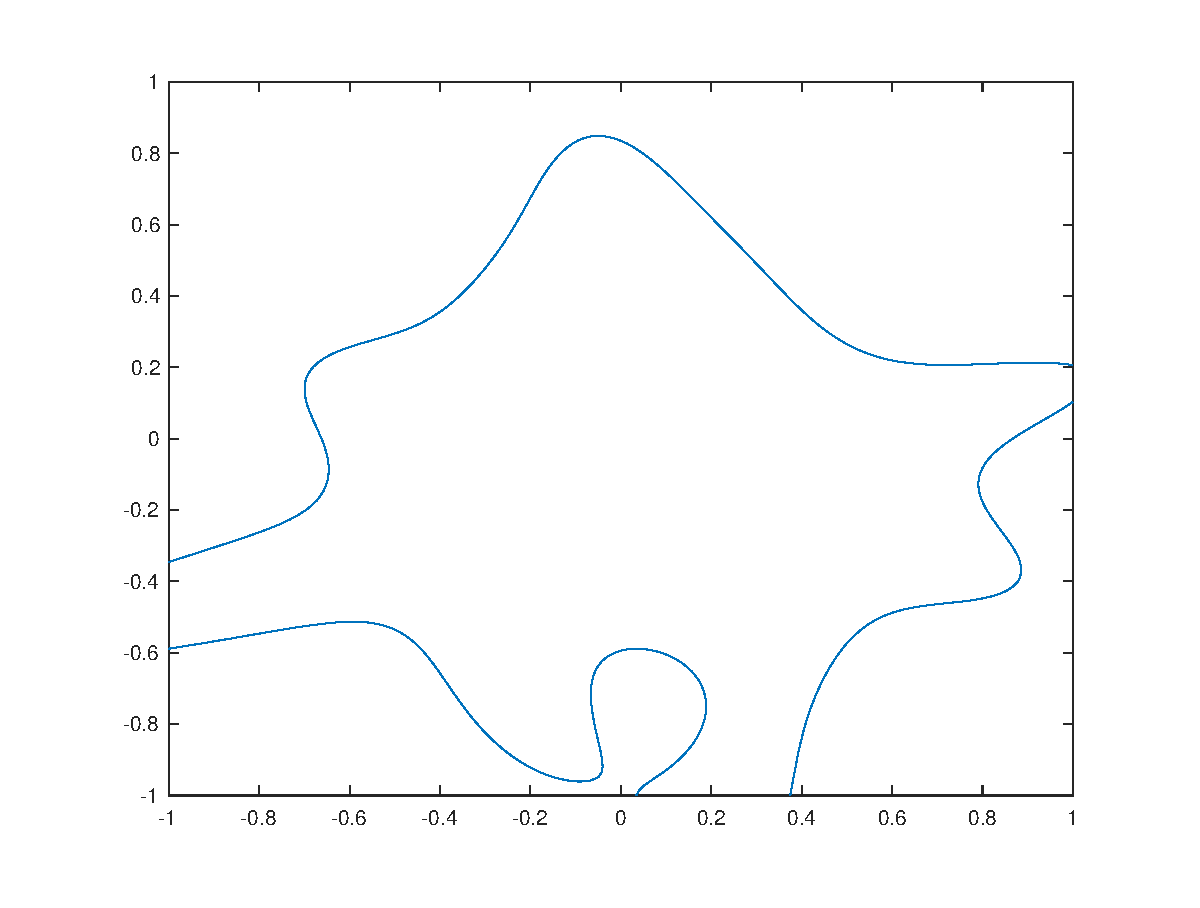
\includegraphics[width=.8\textwidth]{over.eps}
  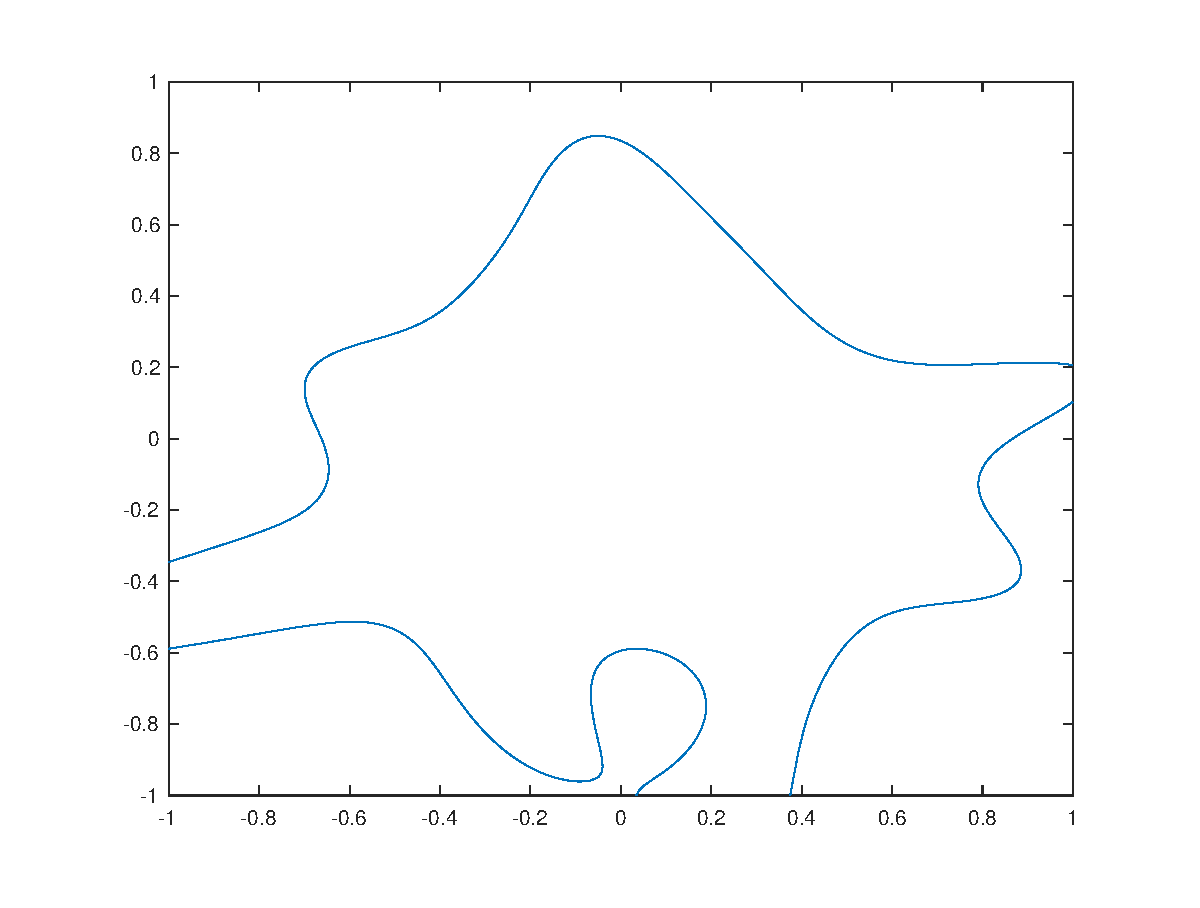
\includegraphics[scale=.8]{over}
  \caption{A plot of the decision boundary for $\lambda = 0$.}
  \label{Fig 1.}
\end{figure}

In the above graph, the horizontal axis is symmetry and the vertical axis intensity. There is no
regularization here, and unsurprisingly the boundary appears to be overfit.

\subsection*{3. Regularization.}

Now, we introduce a lot of regularization.

\begin{figure}[h!]
  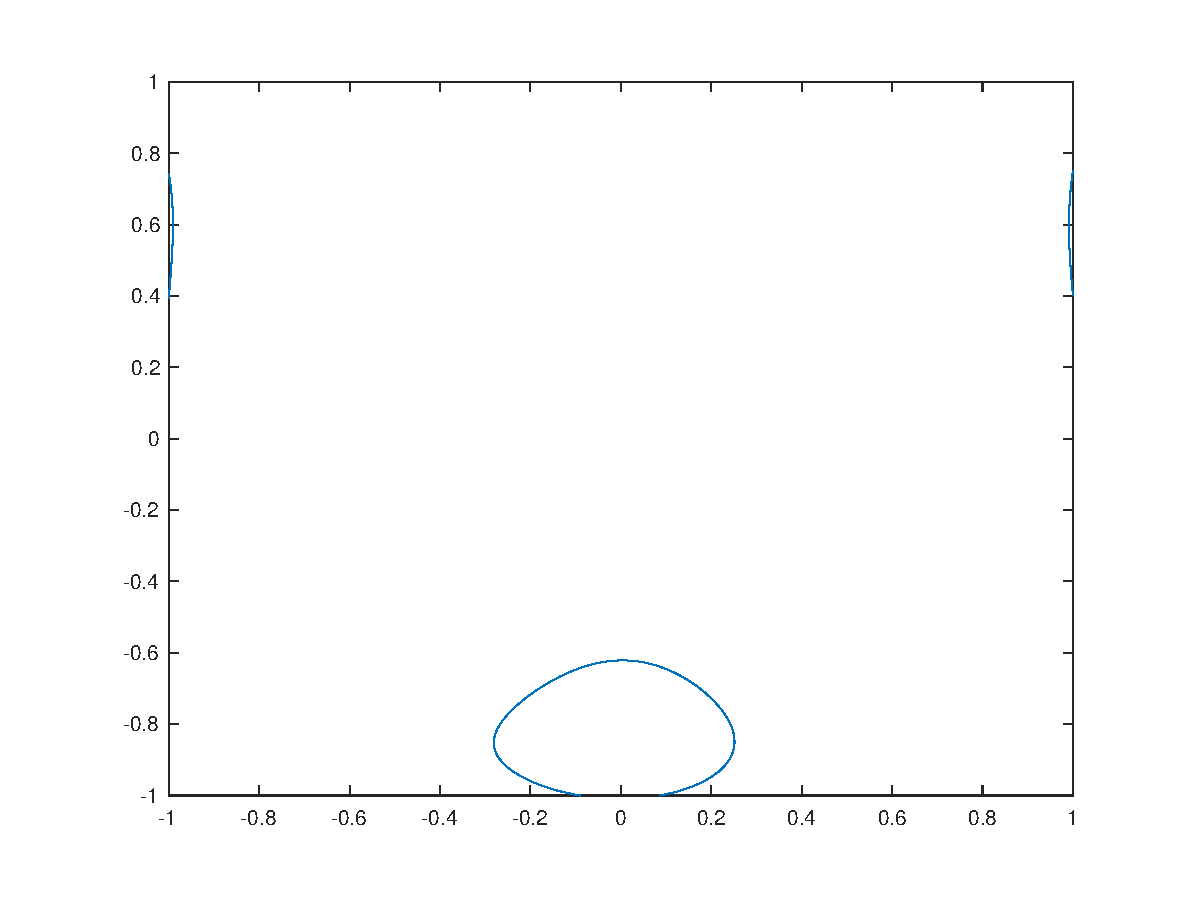
\includegraphics[scale=.8]{under}
  \caption{A plot of the decision boundary for $\lambda = 2$.}
  \label{Fig 2.}
\end{figure}

As expected, there appears to be some underfitting here, with so much regularization.

\subsection*{4. Cross Validation.}

Graphing the cross validation and test errors for each lambda in the range $[0, 2]$, with steps of 
0.01, we have the graph in Figure 3.

As one might guess, the cross validation error is lower than the test error, given that leave-
one-out cross validation still uses essentially the training data. Both have minimums, but at
slightly different lambda values, and both increase somewhat as lambda increases beyond its
apparently optimal value.

\begin{figure}[h!]
  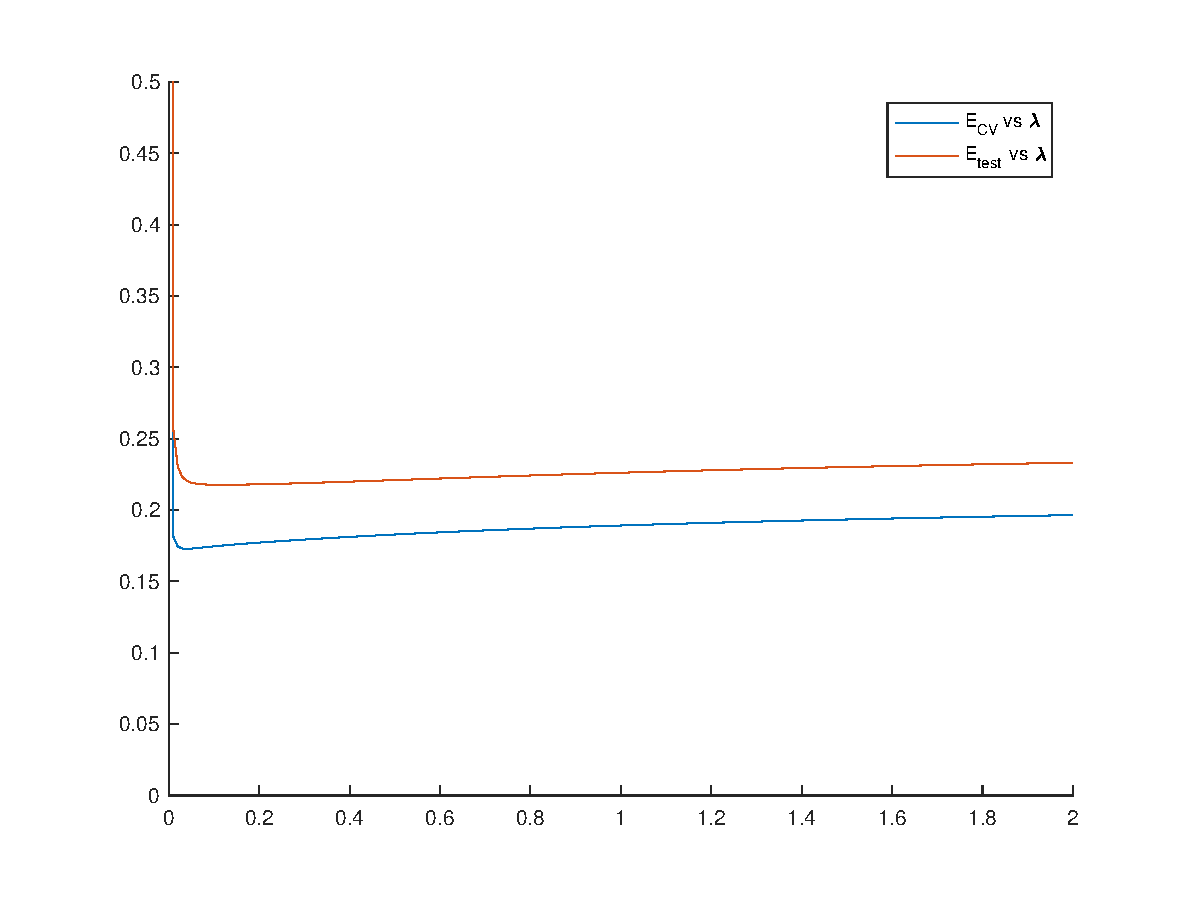
\includegraphics[scale=.8]{errors}
  \caption{The two error measures calculated for $\lambda \in {0, 0.01, 0.02, \dots, 2}$.}
  \label{Fig 3.}
\end{figure}

\subsection*{5. Pick $\lambda$.}

The value chosen for lambda based on the error measures is $$\lambda^* = .04$$ Figure 4 plots
the decision boundary given by $\vec{w}_{reg}(\lambda^*)$.

\begin{figure}[h!]
  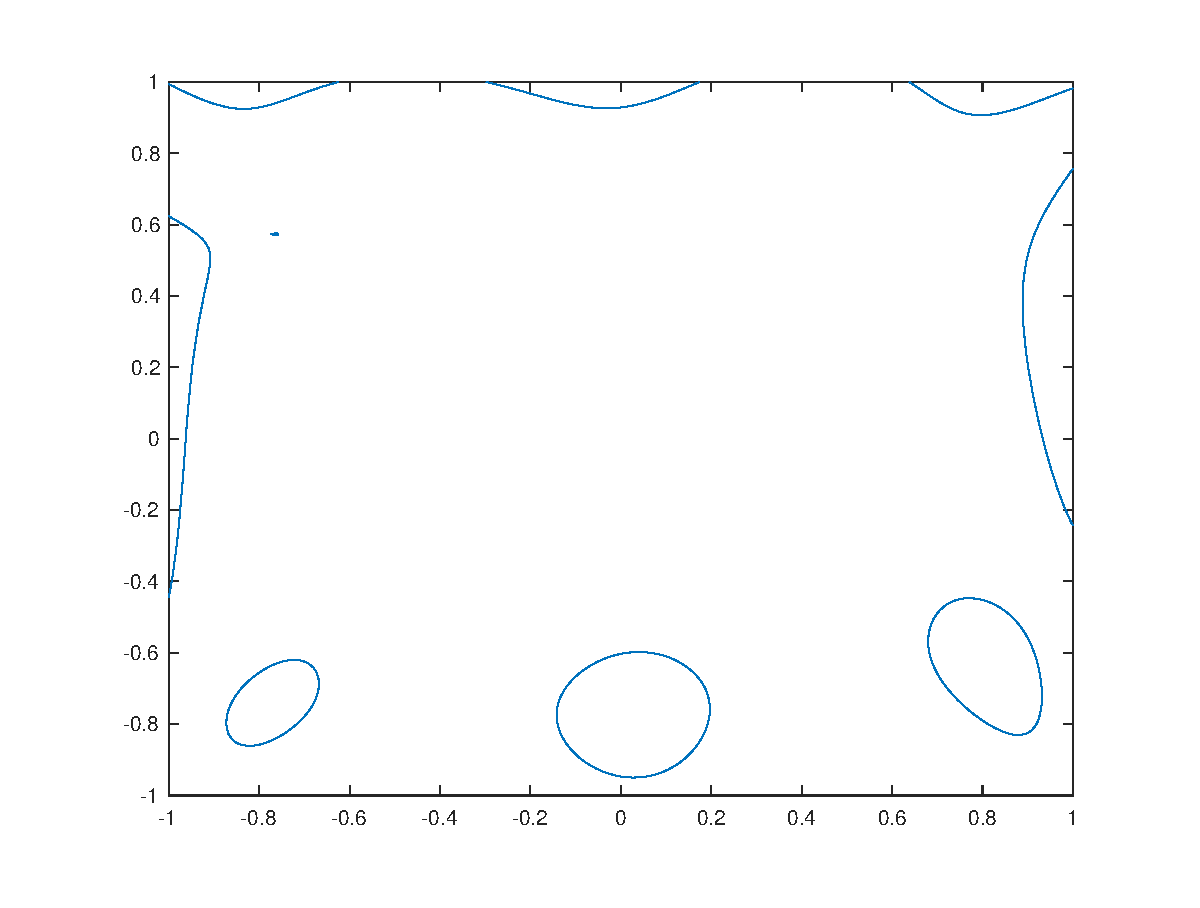
\includegraphics[scale=.8]{final}
  \caption{The final decision boundary, using the $\lambda^*$ obtained from the error}
  \label{Fig 4.}
\end{figure}

\bigskip

\bigskip

\subsection*{6. Estimate $E_{out}$.}

The estimate for $E_{out}$ is simply given by $E_{test}$, for which we have the value $0.0670$.
Thus,

$$E_{out} \approx .0670 = 6.70\%$$

\subsection*{7. Is $E_{CV}$ unbiased?}

$E_{CV}$ is very close to an unbiased estimate of $E_{test}(\vec{w}_{reg}(\lambda^*))$. Because 
of the leave-one-out cross validation, it is a nearly unbiased estimate of $E_{test}$ for each 
one left out, and as we're taking the average of a large set (for each data point left out), we 
get an unbiased estimate.

\subsection*{8. Data Snooping.}

$E_{test}(\vec{w}_{reg}(\lambda^*))$ is not an unbiased estimate of 
$E_{out}(\vec{w}_{reg}(\lambda^*))$ due to data snooping in the normalization of features. 
Normalization of features can only be done when the features are decided and the values known, 
so the data is essentially altered before any learning is done. This is a form of data snooping
and results in bias in the estimate. To fix this problem, you could either not normalize the 
features, or normalize them afterward, not looking at the data before hand, resulting in an 
unbiased estimate.




\end{document}
